
\begin{frame}{}
    \centering\large\textbf{Language Models}
\end{frame}



% ERASE ALL ?

\begin{frame}{Language Models}
      \small 
    
    \begin{definitionBlock}{Definition}
    A \alert{\textbf{language model}} takes a sequence of word vectors and outputs a sequence of predicted word vectors by learning a probability distribution over words in a vocabulary.
    
    They predict words sequentially, unidirectionally, one token at a time, using some context words. 
    
    
    \end{definitionBlock}
    
    Formally, they compute the conditional probability of a word $w_t$ given a context, such as its previous $n-1$ words, where the probability is: $P(w_t \; | \; w_{t-1}, ..., w_{t-n+1})$
    
\end{frame}





% ERASE: 
\begin{frame}{} %{Types of Language Models}



\begin{itemizeSpaced}{5pt}
{\color{DimGray}
    \item \textbf{$n$-gram language model: } an $n$-gram is a sequence of $n$ words. The model finds a word's probability based on frequencies of its constituent $n$-grams, taking just preceding $n-1$ words as context instead of the entire corpus. 
    
    \item \textbf{neural network model: } uses a linear $W \cdot x + b$ function called a neuron. By applying a nonlinear function $f(\cdot)$ to this equation and by incorporating many hidden layers and by stacking neurons together, a neural network can model any function.
    
    Has \textbf{embedding layer}, \textbf{intermediate layers} to transform embeddings, and \textbf{final layer}, which often uses softmax function to normalize word embedding matrix to create probability distribution over words. 
    
    \item \textbf{bidirectional language model (biLM): } calculates probability of a token given its \emph{forward} and \emph{backward} tokens. Uses \textbf{forward} and \textbf{backward language model}s, respectively. 
}% end grey color
\end{itemizeSpaced} 
    

    \begin{figure}[h]
    \vspace{-15pt}
    \centering
    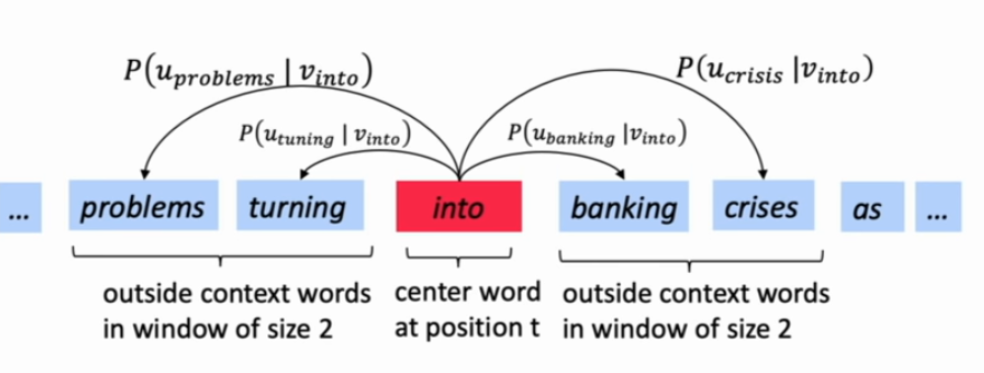
\includegraphics[width=0.65\textwidth]{imgs/bidirectional_languagemodel_banking.png}
    \vspace{-10pt}
    \caption{\tiny Example Bidirectional Language Model. From \emph{Word2Vec Overview With Vectors}, by CS224n: Natural Language Processing with Deep Learning (Stanford), 2018. \url{https://sangminwoo.github.io/2019-08-28-cs224n-lec1/}. Copyright n.d. by n.d.}
    \vspace{-5pt}
    \label{fig:bidirectionalLM}
    \end{figure}
    


\end{frame}





% ERASE
% \begin{frame}{Example: Bidirectional Language Model}
% 
% 
% {\large \textbf{Consider the two sentences ...}
% 
% 
% \textit{``Mary accessed the bank account.”} 
% 
% \textit{``The swan waded to the bank of the river.”}
% 
% }
% 
% \begin{alertBlock}{Warning}
%     \large 
%     A unidirectional contextual model would represent the target word “bank” based on `I accessed the’ but not `account.’ 
%     
%     Cannot capture \textbf{polysemy} of `bank’ !
% \end{alertBlock}
% 
% 
% 
% {\large But a bidirectional language model represents ``bank” using both previous and next context to ameliorate this problem.}
%     
% \end{frame}